% !TEX root = ../YourName-Dissertation.tex
\Appendix{Supportive Data and Figures}

\section{Data}


\section{Figures}
%%%
%%%%%%%%%%%%%%%%%%%%%%%%%%%%%%%%%%
\begin{figure}[H]
    \centering  %居中
    \subfigure[Federal Expenditure]{   %first subfigure
    \begin{minipage}{7cm}
    \centering    %子图居中
    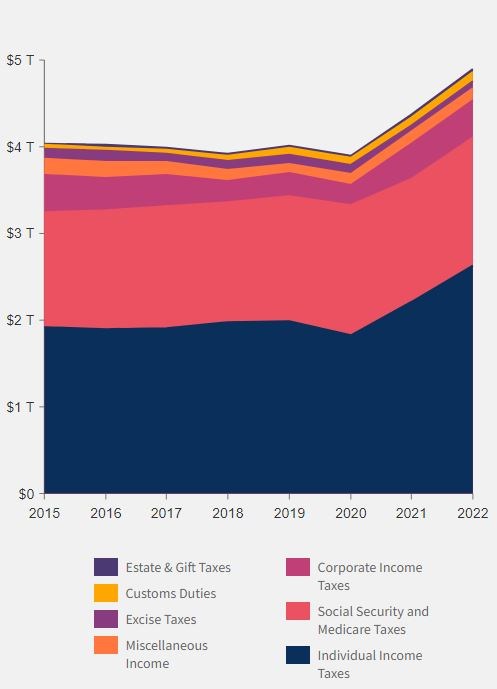
\includegraphics[scale=0.52]{Chapter-1/Figures/source of federal revenue.JPG}  %以pic.jpg的0.5倍大小输出
    \end{minipage}
}
    \subfigure[State and Local Expenditure]{ %second subfigure
    \begin{minipage}{7cm}
    \centering    %子图居中
    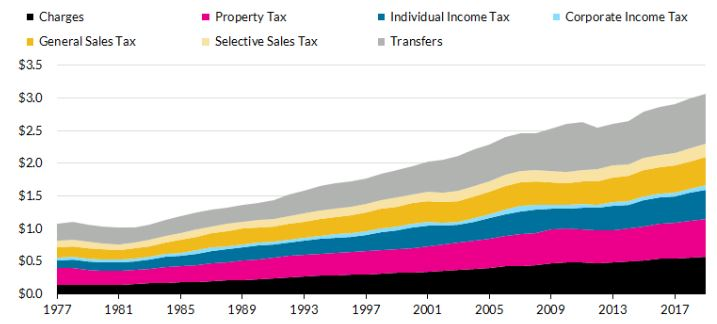
\includegraphics[scale=0.52]{Chapter-1/Figures/source of state and local revenue.JPG}%以pic.jpg的0.5倍大小输出
    \end{minipage}
}
   
    \caption[Fluctuation of Revenue Structure]{Fluctuation of Revenue Structure of three level governments.Data Source: US Urban Institute Dataset  }    %caption for whole figure
    \label{Figure A.1}    
    \end{figure}
